\chapter{Implementierung der Webadministration}
\label{cha:impl_web}

Die Web Administration stellt die zentrale Kontrolleinheit des gesamten Projekts dar. Über die Web Administration werden sämtliche Einträge der Datenbank verwaltet, dies schließt neben der Benutzer- und Geräteverwaltung ebenfalls die Verwaltung aller Regale und Produkte ein.


\section{Technologische Grundlagen}

Die Administrationsoberfläche ist als Webapplikation und im Speziellen als Single-Page-Applikation konzipiert, d.h. sie besteht grundlegend aus einer einzigen Webseite, deren Layout (wie für Webseiten üblich) auf \ac{HTML} und \ac{CSS} aufgebaut ist. Die einzelnen Ansichten (Views) der Anwendung sowie jegliche dynamische Interaktionsprozesse werden über \acl{JS} als clientseitige Scriptsprache gesteuert. Dabei werden auch Daten oder Views im Hintergrund asnychron über \ac{AJAX} nachgeladen. Durch dieses Grundkonzept werden viele Ladevorgänge der kompletten Webseite vermieden und nur die Daten nachgeladen, die im Einzelnen benötigt werden -- dies sorgt für eine bessere Performance der Anwendung und somit eine bessere User Experience.

Das Layout selbst ist \emph{responsive}, d.h. es passt sich flexibel an die gegebene Bildschirmgröße des Ausgabegerätes durch eine optimiertes Layout (veränderte Anordnung von Seitenelementen, optimierte Platznutzung) an. Dadurch ist die Webadministration nicht nur für die Nutzung am Desktop-PC und großen Bildschirmen, sondern auch für die Verwendung auf Tablets und Smartphones gerüstet, sollte die Webanwendung im gesamten Netzwerk verfügbar sein (siehe Architektur).

Wie bereits in der Architektur angedeutet, läuft die Webadministration serverseitig mit der Scriptsprache \ac{PHP}. Hierüber werden Inhalte und Layoutkomponenten vorgeneriert und abhängig von den Parametern der clientseitigen Anfragen ausgeliefert. Auch die Validierung von Formularanfragen, sowie die Verbindung zur Datenbank und Datenbank-Abfragen werden über \ac{PHP} durchgeführt. Für die Datenbank selbst wird wegen der guten Kompatibilität mit PHP auf MySQL gesetzt.

Unter bestimmten Bedingungen (z.B. Sicherheitsvorschriften oder technische Einschränkungen) könnte die Ausführung von JavaScript im Browser des Anwenders nicht möglich sein. Die Webadministration ist in ihrer Funktionalität zu einem großen Teil auch ohne aktiviertes \acs{JS} lauffähig, indem die statischen Fallback-Links und Standardfunktionalitäten greifen, die via JavaScript sonst geblockt und eigene Interaktionsmethoden ersetzt werden. Dennoch lassen sich Teile der Anwendung ohne Einsatz von JavaScript nur sehr aufwändig umsetzen; als Beispiel dafür sei hier der Shelf Designer genannt, der im Folgenden noch näher beschrieben wird und ohne \acs{JS} nicht funktionsfähig ist.


\section{Bereiche und Funktionen}

Das Layout der Webadministration ist in eine Navigationsleiste, eine Subnavigation und einen Inhaltsbereich aufgeteilt. Über die Navigationsleiste können die funktionalen Hauptbereiche geöffnet werden, die jeweils in der Subnavigation noch über Unterseiten verfügen. Der Inhaltsbereich enthält häufig Tabellen, die rechts eine Spalte mit Buttons für Aktionen zu einem Eintrag der Tabelle bereit halten. Tabellen, die wegen einer hohen Anzahl an Einträgen sehr lang werden würden, werden dabei automatisch auf mehrere Seiten verteilt, die über eine dann eingeblendete Seitennavigation geöffnet werden können. Die restlichen Views sind i.d.R. Formulare (z.B. für \emph{Neue Produkt anlegen} oder, bereits vorausgefüllt, \emph{Produkt bearbeiten}).

In den folgenden Kapiteln sollen die Bereiche der Webadministration ausführlich vorgestellt werden. Auf eine detaillierte Aufführung der betroffenen Daten und Felder wird dabei zwecks Übersichtlichkeit verzichtet -- diese wurden bereits in der Datenbank-Architektur (Kapitel \ref{sec:architektur_datenbank}) genauer erläutert.

\subsection{Produkte \& Einheiten}

\begin{figure}[H]
	\centering
	{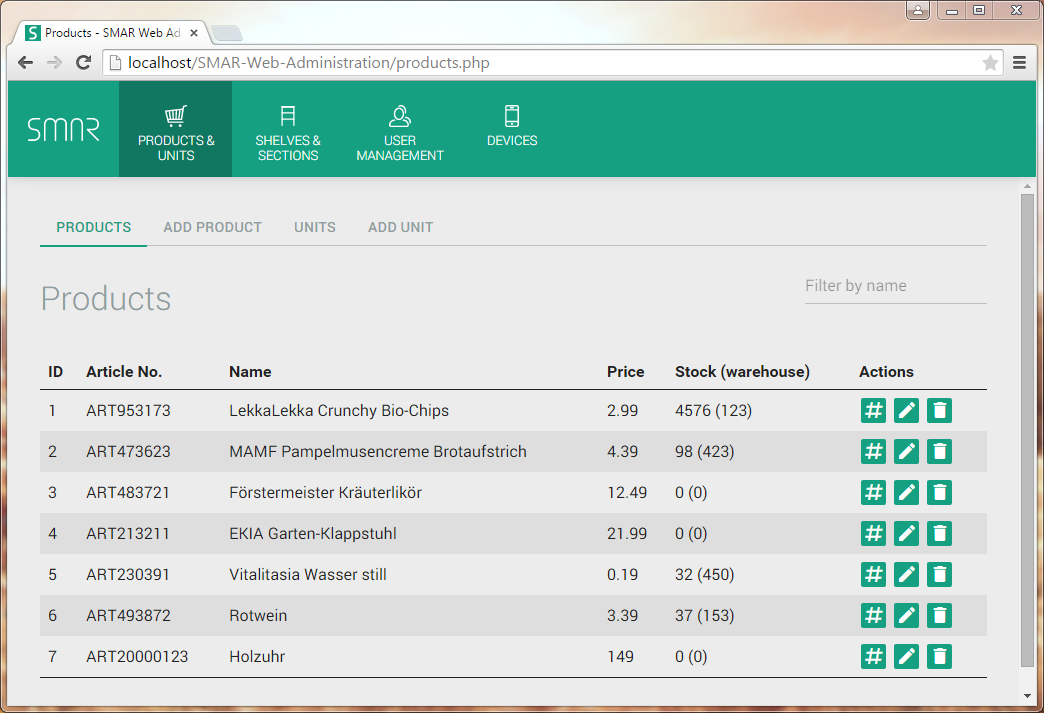
\includegraphics[width=\textwidth]{Bilder/Abbildungen/webadmin_products.png}}
	\caption{Produktübersicht in der Webadministration (Screenshot)}
	\label{fig:webadmin_products}
\end{figure}

In diesem Abschnitt können alle wesentlichen Aspekte rund um Produkte und die Einheiten, in denen Produkte auftreten können, verwaltet werden.\\

Als erstes wird eine Produktübersicht in Listenform angezeigt, über welche alle vorhandenen Produkte gefunden werden können. Zu einem Produkt werden die wesentlichen Informationen angezeigt, um ein Produkt identifizieren zu können, sowie der aktuelle Warenbestand eines Produktes. Über die Aktionen kann ein Produkt bearbeitet oder gelöscht werden, sowie die entsprechenden Produkt-Einheiten-Mappings angezeigt werden, die im Folgenden noch erläutert werden.\\

Auf einer Unterseite, erreichbar über die Subnavigation, kann über ein Formular ein neues Produkt angelegt werden, indem die notwendigen Informationen angegeben werden. Die notwendigen Abhängigkeiten zu anderen Tabellen werden dabei von der Webadministration automatisch angelegt. Analog gibt es ein Formular zum Anlegen von Einheiten für Produkte.\\

Zur Anzeige der vorhandenen Produkteinheiten gibt es eine Einheitenliste in einem eigenen View. Dieser gleicht (bis auf die dargestellten Informationen zu Einheiten) genau der Produktübersicht. In der Einheitenübersicht können ebenso einzelne Einträge betrachtet, bearbeitet und gelöscht werden; außerdem können auch hier für einzelne Einheiten die entsprechenden Produkt-Einheiten-Mappings angezeigt werden.\\

Ein nicht über die Subnavigation zugänglicher View sind die Produkt-Einheiten-Mappings. Diese Ansicht öffnet sich, wenn sie über die Produkt- oder Einheitenliste ausgewählt wird, und zeigt auf, welche Einheiten einem Produkt zugeordnet sind. In diesem View können die Zuordnungen auch bearbeitet, sowie neue Zuordnungen hinzugefügt werden. Die Produkt-Einheiten-Mappings sind z.B. wichtig zur Erkennung von Kartons, die eine größere Menge eines Produktes enthalten. Für diesen Zweck kann ein eigener Barcode pro Produkt-Einheit-Mapping gespeichert werden.


\subsection{Regale \& Fächer}


\subsection{Shelf Designer}

\begin{figure}[H]
	\centering
	{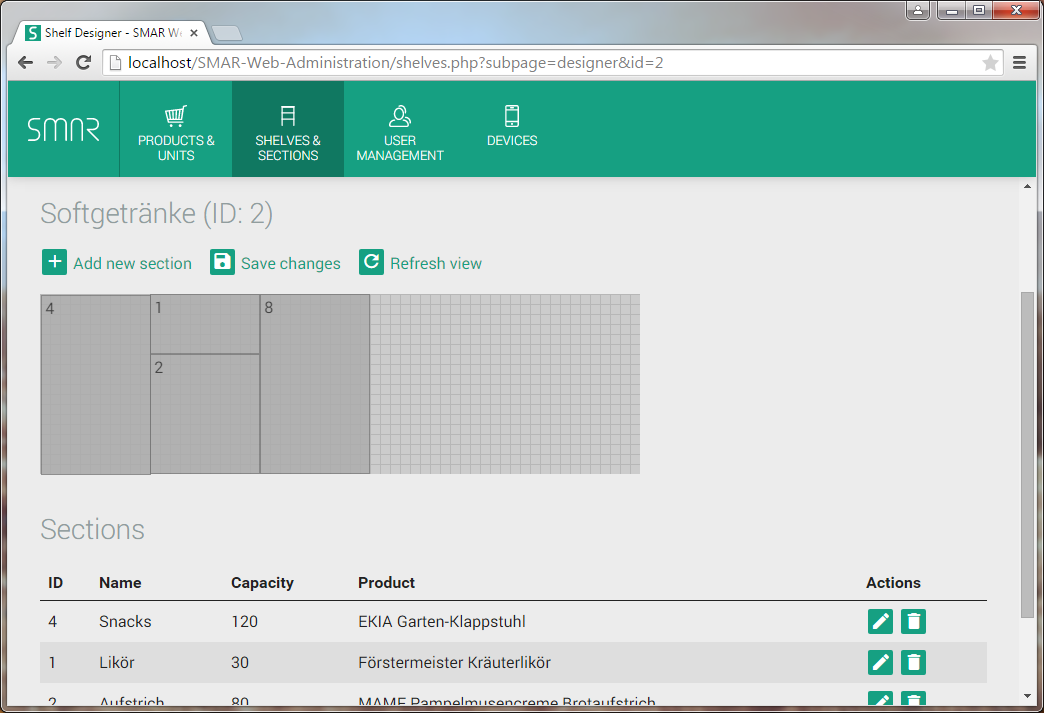
\includegraphics[width=\textwidth]{Bilder/Abbildungen/webadmin_shelves_designer.png}}
	\caption{Shelf Designer in der Webadministration (Screenshot)}
	\label{fig:webadmin_shelves_designer}
\end{figure}


\subsection{Benutzerverwaltung}

%TODO Sebastian

\subsection{Weitere Funktionen}
Nicht implementiert: Market Map und Map Designer, Bestellungen

\chapter{Implementierung der Client-Schnittstelle}

REST API

Slim Framework (Implementierung)

%TODO: Erläutern, warum Berechnung der Kapazität abgelehnt wird


